%!TEX root = ../thesis.tex

\section{経路追従}
経路追従(Path following)とは, 経路計画(Path planning)で引いた経路に対して安全にロボットが経路を追従できるようにロボットを制御することである.
基本的にはロボットのモデルと制御アルゴリズムを利用することで, 最終的にロボットの入力値(ステアリング角度や並進速度)を計算することが目的となる.

\subsection{PurePursuit}
PurePursuitアルゴリズムは, 経路追従アルゴリズムの中で最も基礎的だが, 非常に広く使われているアルゴリズムである.

PurePursuitはFig.3.1に示すように目標経路上(Path)に対して一定距離先の点を目標点(Look Ahead)とし, その点に到達するようなステアリング制御を行う.
目標点に対してロボットが前進することで, より先の目標点にたどり着くように制御を行うため, 結果的に目標経路に追従する形となる.

\begin{figure}[H]
  \centering
 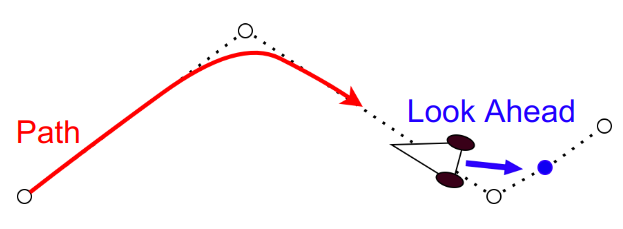
\includegraphics[keepaspectratio, scale=0.5]
      {images/PurePursuit.png}
 \caption{PurePursuit Algorithm}
 \label{fig:purepursuit}
\end{figure}

\subsection{PID制御}
PID制御(Proportional-Integral-Differential Controller)は, 制御工学におけるフィードバック制御の一種である.
出力値と目標値との偏差, その積分, および微分の3つの要素によって, 入力値の制御を行う方法である.



\newpage